\documentclass[twoside,11pt]{homework}
\usepackage{graphicx}
\usepackage{booktabs}
\usepackage{lipsum}
\usepackage{indentfirst}
\usepackage{algorithm}
\usepackage{algorithmic}
\usepackage{makecell}
\usepackage{indentfirst}
\usepackage{bbm, dsfont}

\coursename{COMS 4771 Machine Learning (Spring 2015)} % DON'T CHANGE THIS

\studname{Jingwei Yang}    % YOUR NAME GOES HERE
\studmail{jy2653@columbia.edu}% YOUR UNI GOES HERE
\hwNo{4}                   % THE HOMEWORK NUMBER GOES HERE
\collab{pp2526,yd2300}   % THE UNI'S OF STUDENTS YOU DISCUSSED WITH
\begin{document}
\maketitle

\section*{Problem 1}
\indent
(a)
\begin{align*}
\mathbb{E}[(Y - \hat Y) ^ 2] &= \mathbb{E}[(Y - \langle \pmb w, \pmb X \rangle ) ^ 2] 
\end{align*}
Take a gradient of $\pmb w$
\begin{align*}
\nabla_ {\pmb w} \mathbb{E}[(Y - \langle \pmb w, \pmb X \rangle ) ^ 2] = \mathbb{E} [2 (Y - \langle \pmb w, \pmb X \rangle )  \pmb X ^ T ]\\
\end{align*}
To minimize $\mathbb{E}[(Y - \hat Y) ^ 2] $, the $\nabla_ {\pmb w} \mathbb{E}[(Y - \langle \pmb w, \pmb X \rangle ) ^ 2]$ should equal to 0, then we have
\begin{align*}
\pmb w^T \pmb X \pmb X ^ T &= Y \pmb X ^ T \\
\pmb w ^ T &= (Y \pmb X ^ T) (\pmb X \pmb X ^ T) ^ {-1} \\
\pmb w &=  (\pmb X \pmb X ^ T) ^ {-1} (\pmb X  Y) 
\end{align*}


(b) \\
\begin{align*}
\mathbb{E} [(Y - \langle \pmb w, \pmb X \rangle ) \pmb X]  & =  \mathbb{E} [(Y -  \pmb w ^ T \pmb X) \pmb X] \\
& = \mathbb{E} [(Y - Y \pmb X ^ T (\pmb X \pmb X ^ T) ^{-1} \pmb X) \pmb X] \\
& = \mathbb{E} [(Y - Y \pmb X ^ T  (\pmb X ^ T) ^ {-1} \pmb X ^ {-1} \pmb X) \pmb X] \\
& = \pmb 0
\end{align*}


(c) \\
\begin{align*}
\mathbb{E}[Z_i \pmb X_{(-i)}]  &= \mathbb{E} [X_i \pmb X_{(-i)} - E(X_i \pmb X_{(-i)} )^T E(\pmb X_{(-i)} \pmb X^T_{(-i)})^{-1}\pmb X_{(-i)}\pmb X_{(-i)}]\\
& =  \mathbb{E} [X_i \pmb X_{(-i)} - X_i \pmb X_{(-i)} ^T ( \pmb X_{(-i)}^T)^{-1} \pmb X_{(-i)}^{-1} \pmb X_{(-i)} \pmb X_{(-i)} ] \\
& = \pmb 0
\end{align*}

(d) \\
\begin{align*}
\mathbb{E}[Z_i ^2] &= \mathbb{E}[Z_iX_i - Z_i X_i \pmb X_{(-i)}^T (\pmb X_{(-i)} \pmb X_{(-i)}^T)^{-1} \pmb X_{(-i)}] \\
& = \mathbb{E} [Z_iX_i - X_i \pmb X_{(-i)}^T (\pmb X_{(-i)} \pmb X_{(-i)}^T)^{-1} Z_i \pmb X_{(-i)}] \\
& =  \mathbb{E} [Z_iX_i - X_i \pmb X_{(-i)}^T (\pmb X_{(-i)} \pmb X_{(-i)}^T)^{-1} \pmb 0] \\
& = \mathbb{E} [Z_iX_i ]
\end{align*}


\begin{align*}
 \mathbb{E}[\langle \pmb w, \pmb X \rangle  Z_i] &=  \mathbb{E}[(\langle \pmb w_{(-i)}, \pmb X_{(-i)} \rangle  + w_i X_i )Z_i] \\
 & = \mathbb{E}[Z_i \pmb X_{(-i)} \pmb w_{(-i)} ^T+ w_i X_i Z_i] \\
  & = \mathbb{E}[0 + w_i X_i Z_i] \\
 & = w_i  \mathbb{E}[Z_iX_i]
\end{align*}

\begin{align*}
\mathbb{E}[(Y - \hat Y)Z_i] &= \mathbb{E}[(Y - \hat Y)X_i - (Y - \hat Y)X_i \pmb X_{(-i)}^T (\pmb X_{(-i)} \pmb X_{(-i)}^T)^{-1} \pmb X_{(-i)}]\\
\end{align*}

According to part (b), we know $\mathbb{E}[(Y - \hat Y)\pmb X] = \pmb 0 $, thus $\mathbb{E}[(Y - \hat Y)X_i = 0$. Thus we have 
\begin{align*}
\mathbb{E}[(Y - \hat Y)Z_i] = 0
\end{align*}


Since 
\begin{align*}
\mathbb{E} [YZ_i] = \mathbb{E} [\langle \pmb w, \pmb X \rangle Z_i + (Y - \hat Y) Z_i]
\end{align*}


thus 
\begin{align*}
\mathbb{E} [YZ_i]  = w_i  \mathbb{E}[Z_iX_i] = \mathbb{E}[Z_i ^2] w_i
\end{align*}





% YOUR SOLUTION GOES HERE
\section*{Problem 2}
(a)
As we can see from following comparision, the quantized  image at k = 64 has better approximated performance than that at k = 8. Cause when k = 64, we could have more representative patches to choose from, thus the approximated performance is more refined. 

\begin{center}
\textbf{image 24, k = 8}\par\medskip
\includegraphics[width=150mm, height = 80mm]{image-24,k-8.eps}
\end{center}

\begin{center}
\textbf{image 24, k = 64}\par\medskip
\includegraphics[width=150mm, height = 80mm]{image-24,k-64.eps}
\end{center}

\newpage


\begin{center}
\textbf{image 100, k = 8}\par\medskip
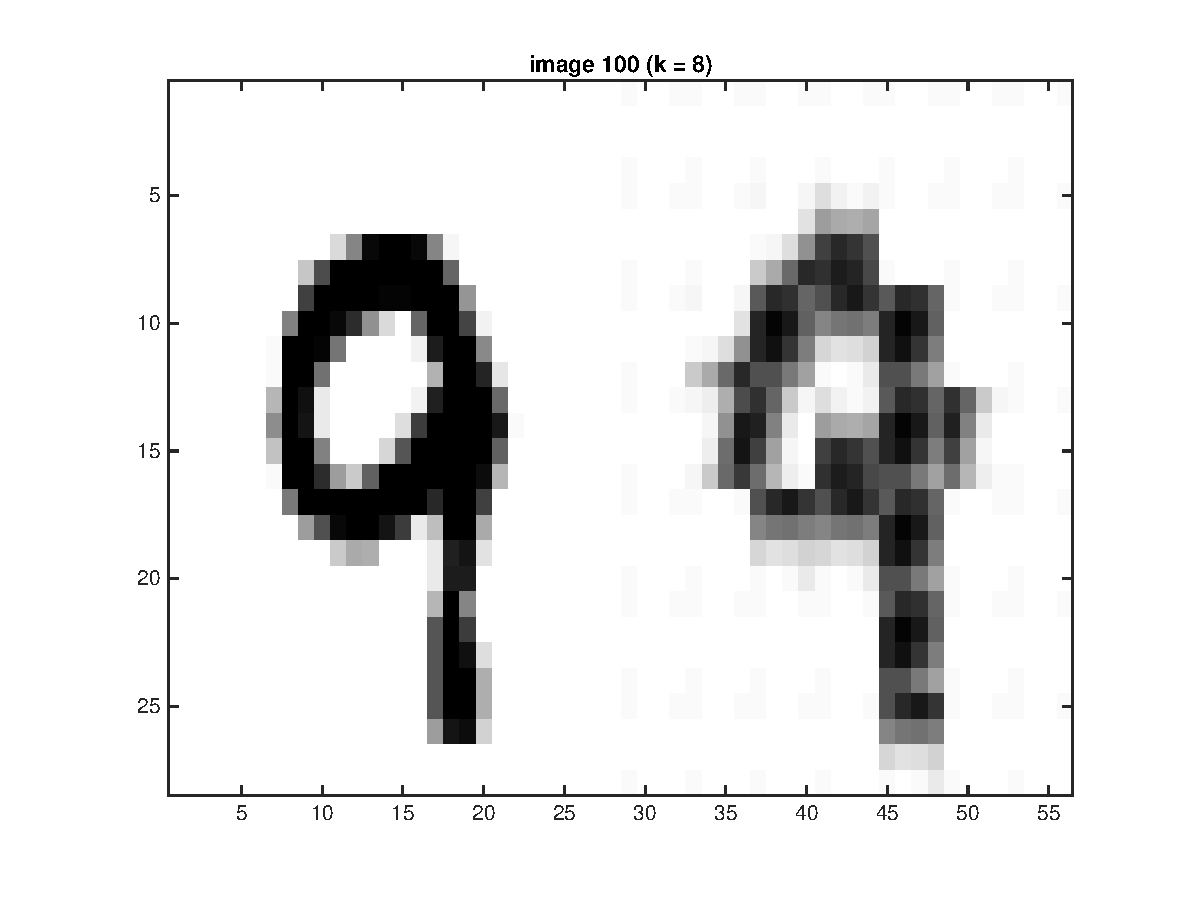
\includegraphics[width=150mm, height = 80mm]{image-100,k-8.eps}
\end{center}

\begin{center}
\textbf{image 100, k = 64}\par\medskip
\includegraphics[width=150mm, height = 80mm]{image-100,k-64.eps}
\end{center}

\newpage


\begin{center}
\textbf{image 5000, k = 8}\par\medskip
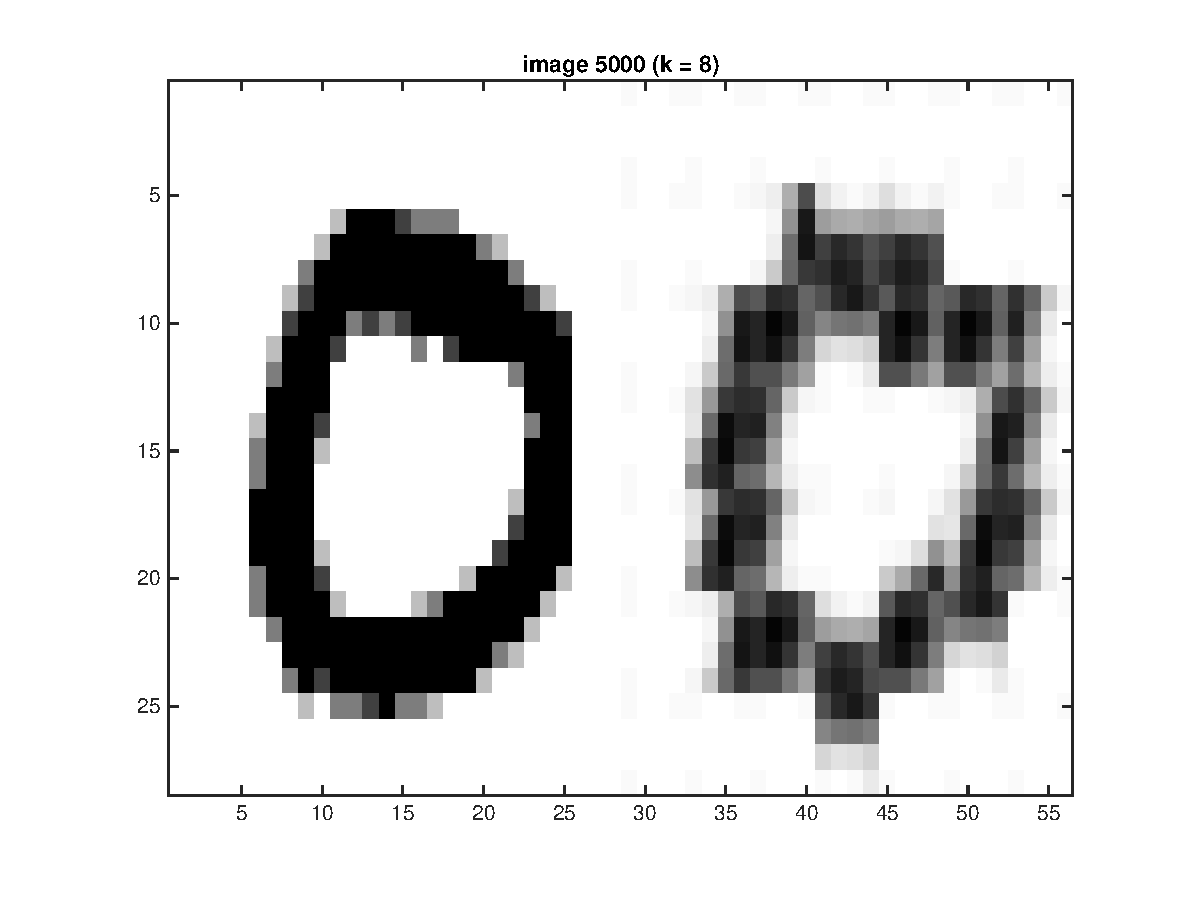
\includegraphics[width=150mm, height = 80mm]{image-5000,k-8.eps}
\end{center}


\begin{center}
\textbf{image 5000, k = 64}\par\medskip
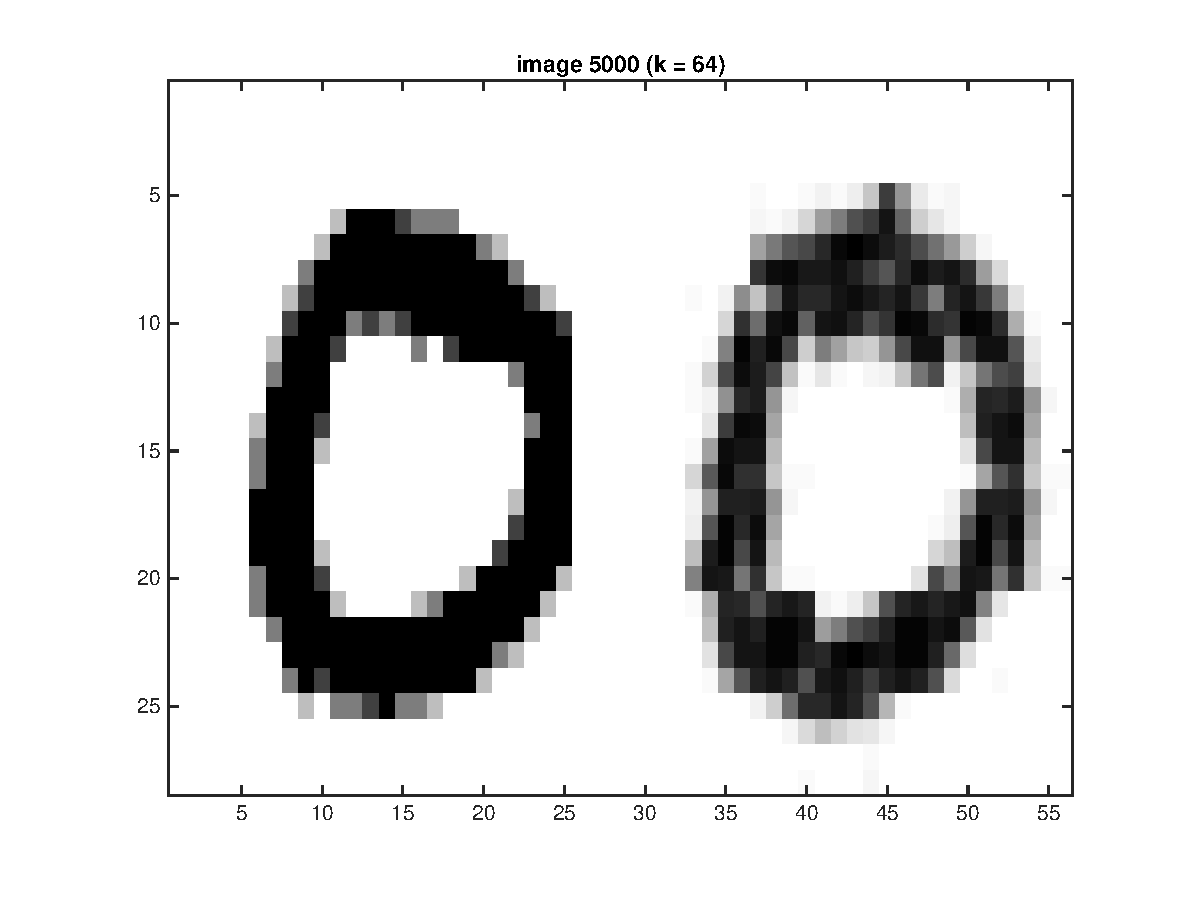
\includegraphics[width=150mm, height = 80mm]{image-5000,k-64.eps}
\end{center}

\newpage

(b) \\ \indent
$f(k) = (16 * k + 10000 * 49) * 64$ \\ \indent
Assume we use 64-bit integer numbers to record the indexes of each representative for each image. \\
Reasoning: \\ \indent
Each patch is a $4 * 4$ matrix, thus we need to use 16 double to record a patch (16 double-precision floating point numbers), $16 * k$ is the number of double-precision floating point numbers needed for recording all representative patches. \\ \indent
After quantization, we only need to record a $7 * 7$ matrix for each image,  which is 49 64-bit integer numbers. Since we have 10000 test images in total,  we need to use $10000 * 49$ 64-bit integer numbers to record all quantized images. \\ \indent
Since each double-precision floating point number use 64 bits, the total bits needed is $f(k) = (16 * k + 10000 * 49) * 64$.\\


(c) \\ \indent
\begin{center}
\textbf{cost curve for online K-means algorithm}\par\medskip
\includegraphics[width=150mm, height = 80mm]{cost_curve.eps}
\end{center}












% YOUR SOLUTION GOES HERE
\section*{Problem 3}
sfdsdf\\
$\ell_{sq} (z) = (1 - z) ^ 2$ \\
$\ell_{log}(z) = \ln (1 + \exp (-z))$\\
$\ell_{\exp}(z) = \ln (\exp (-z))$ \\



(a) \\
Since $Y$ in $\{-1, +1\}$, $\ell_{sq} (Y \hat y) = (1 - Y\hat y) ^ 2$.
When $Y = +1$, $\ell_{sq}(Y\hat y) = (1- \hat y)^2$, 
When $Y = -1$, $\ell_{sq}(Y \hat y) = (1+ \hat y)^2$ .
And $Pr(Y = +1) = \eta$, $Pr(Y= -1) = 1 - \eta $. We have 
\begin{align*}
\mathbb{E}[\ell_{sq} (Y \hat y)] = \eta(1-\hat y)^2 + (1-\eta) (1+ \hat y)^2
\end{align*}
Take the gradient of $\hat y$, we have \\
\begin{align*}
\nabla _ {\hat y} \mathbb{E}[\ell_{sq} (Y \hat y)] &= 2\eta (\hat y -1) + 2(1- \eta) (1+ \hat y) \\
& = 2\eta \hat y - 2\eta +2 +2\hat y - 2\eta - 2\eta \hat y \\
& = 2 - 4\eta + 2\hat y
\end{align*}
Since $\ell_{sq} (Y \hat y) = (1 - Y\hat y) ^ 2$ is a convex function, to minimize $\mathbb{E}[\ell_{sq} (Y \hat y)]$, we assign $\nabla _ {\hat y} \mathbb{E}[\ell_{sq} (Y \hat y)] = 0$, thus we have 
$\hat y= 2\eta -1 $ \\




(b) \\
Since $Y$ in $\{-1, +1\}$, $\ell_{log}(Y \hat y) = \ln (1 + \exp (-Y\hat y))$.
When $Y = +1$, $\ell_{log}(Y\hat y) =  \ln (1 + \exp (-y))$.
When $Y = -1$, $\ell_{log}(Y \hat y) = \ln (1 + \exp (y))$.
And $Pr(Y = +1) = \eta$, $Pr(Y= -1) = 1 - \eta $. We have 
\begin{align*}
\mathbb{E}[\ell_{log} (Y \hat y)] = \eta \ln (1 + \exp (-\hat y)) + (1-\eta) \ln(1 + \exp (\hat y))
\end{align*}
Take the gradient of $\hat y$, we have \\
\begin{align*}
\nabla _ {\hat y} \mathbb{E}[\ell_{log} (Y \hat y)]  &= \eta \frac {-\exp(-\hat y)}{1+\exp(-\hat y)} + (1 - \eta) \frac {\exp({\hat y})}{1 + \exp ({\hat y})}
\end{align*}
Since $\ell_{log}(Y \hat y) = \ln (1 + \exp (-Y\hat y))$ is a convex function , to minimize $\mathbb{E}[\ell_{log} (Y \hat y)]$, we assign $\nabla _ {\hat y} \mathbb{E}[\ell_{log} (Y \hat y)] = 0$, thus we have
\begin{align*}
 \frac {\eta \exp(-\hat y)}{1+\exp(-\hat y)} = \frac {(1 - \eta)\exp({\hat y})}{1 + \exp ({\hat y})} \\
 \end{align*}
 $\implies$ 
 \begin{align*}
\eta \exp(-\hat y) + \eta = \exp (\hat y) - \eta \exp(\hat y) + 1 - \eta
 \end{align*}
  $\implies$ 
\begin{align*}
\frac{\eta \exp(\hat y) + \eta}{\exp (\hat y)} = (\exp(\hat y) + 1)(1 - \eta)
\end{align*}
 $\implies$ 
\begin{align*}
\eta = \exp(\hat y) (1- \eta)
\end{align*}
 $\implies$ 
\begin{align*}
\hat y = \ln \frac{\eta}{1 - \eta}
\end{align*}

Thus when $\hat y = \ln \frac{\eta}{1 - \eta}$, ${E}[\ell_{log} (Y \hat y)]$ is minized. \\


(c) \\
Since $Y$ in $\{-1, +1\}$, $\ell_{\exp}(Y \hat y) = \ln (\exp (-Y\hat y))$.
When $Y = +1$, $\ell_{log}(Y\hat y) = \ln (\exp (- \hat y))$.
When $Y = -1$, $\ell_{log}(Y \hat y) = \ln (\exp ( \hat y))$.
And $Pr(Y = +1) = \eta$, $Pr(Y= -1) = 1 - \eta $. We have 
\begin{align*}
\mathbb{E}[\ell_{\exp} (Y \hat y)] = \eta \exp (-\hat y) + (1-\eta) \exp (\hat y)
\end{align*}
Take the gradient of $\hat y$, we have 
\begin{align*}
\nabla _ {\hat y} \mathbb{E}[\ell_{\exp} (Y \hat y)]  &=  (1- \eta) \exp (\hat y)- \eta \exp (- \hat y) 
\end{align*}
Since $\ell_{\exp}(Y \hat y) = \ln (\exp (-Y\hat y))$ is a convex function, to minimize $\mathbb{E}[\ell_{\exp} (Y \hat y)]$, we assign $\nabla _ {\hat y} \mathbb{E}[\ell_{\exp} (Y \hat y)] = 0$, thus we have
\begin{align*}
\frac {\eta}{\exp(\hat y)} = \exp (\hat y) (1 - \eta )
\end{align*}
$\implies$
\begin{align*}
\exp (2\hat y) = \frac {\eta}{1-\eta}
\end{align*}
$\implies$
\begin{align*}
2\hat y = \ln \frac {\eta}{1-\eta}
\end{align*}
$\implies$
\begin{align*}
\hat y = \frac {1}{2} \ln \frac {\eta}{1-\eta}
\end{align*}
 Thus when $\hat y = \frac {1}{2} \ln \frac {\eta}{1-\eta}$, ${E}[\ell_{\exp} (Y \hat y)]$ is minized. \\
\end{document} 